\documentclass[paper=b4j,landscape,twocolumn,fleqn]{jlreq}
\special{papersize=\the\paperwidth,\the\paperheight}
\setlength{\columnseprule}{0.4pt}
\pagestyle{empty}
\usepackage[margin=10truemm]{geometry}
\usepackage[dvipdfmx]{graphicx}
\usepackage{amsmath}
\usepackage{tikz}
\usepackage{pgfplots}
\usetikzlibrary{arrows,shapes,positioning,calc}

% セクション見出しの設定
\ModifyHeading{section}{
  lines=1,
  before_space=10pt,
  after_space=0pt
}

\begin{document}

\section{座標と距離}
次の2点の距離を求めよ。\\
\begin{minipage}{0.45\columnwidth}
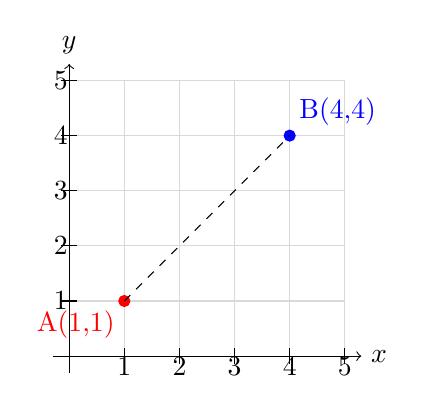
\begin{tikzpicture}[scale=0.7]
  \draw[gray!30] (0,0) grid (5,5);
  \draw[->] (-0.3,0) -- (5.3,0) node[right] {$x$};
  \draw[->] (0,-0.3) -- (0,5.3) node[above] {$y$};
  \foreach \x in {1,2,3,4,5}
    \draw (\x,-0.15) -- (\x,0.15) node[below] {\x};
  \foreach \y in {1,2,3,4,5}
    \draw (-0.15,\y) -- (0.15,\y) node[left] {\y};
  \filldraw[red] (1,1) circle (0.1) node[below left] {A(1,1)};
  \filldraw[blue] (4,4) circle (0.1) node[above right] {B(4,4)};
  \draw[dashed] (1,1) -- (4,4);
\end{tikzpicture}
\end{minipage}
\begin{minipage}{0.45\columnwidth}
A から B までの距離は？\\
$AB = \sqrt{(4-1)^2 + (4-1)^2} = $
\end{minipage}

\section{直角三角形と三角比}
下の直角三角形について，$\sin\theta$，$\cos\theta$，$\tan\theta$ を求めよ。\\
\begin{minipage}{0.4\columnwidth}
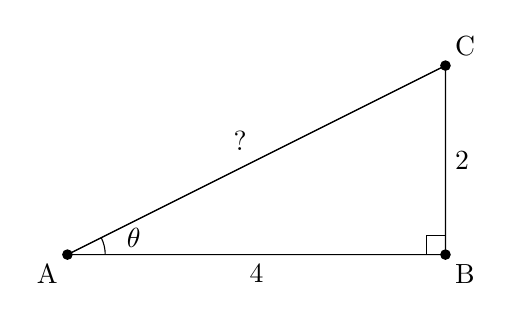
\begin{tikzpicture}[scale=1.2]
  \coordinate (A) at (0,0);
  \coordinate (B) at (4,0);
  \coordinate (C) at (4,2);
  
  \draw (A) -- (B) -- (C) -- cycle;
  \draw (4,0) rectangle (3.8,0.2);
  
  \filldraw (A) circle (0.05) node[below left] {A};
  \filldraw (B) circle (0.05) node[below right] {B};
  \filldraw (C) circle (0.05) node[above right] {C};
  
  \draw (A) -- (B) node[midway,below] {4};
  \draw (B) -- (C) node[midway,right] {2};
  \draw (A) -- (C) node[midway,above left] {?};
  
  \draw (0.4,0) arc(0:26.57:0.4) node[right,xshift=0.2cm] {$\theta$};
\end{tikzpicture}
\end{minipage}
\begin{minipage}{0.55\columnwidth}
斜辺の長さ：$AC = \sqrt{4^2 + 2^2} = $ \\[10pt]
$\sin\theta = \dfrac{対}{斜} = \dfrac{2}{?} = $ \\[10pt]
$\cos\theta = \dfrac{隣}{斜} = \dfrac{4}{?} = $ \\[10pt]
$\tan\theta = \dfrac{対}{隣} = \dfrac{2}{4} = $
\end{minipage}

\section{ベクトルの成分}
下のベクトルの成分表示と大きさを求めよ。\\
\begin{minipage}{0.45\columnwidth}
\begin{tikzpicture}[scale=0.9]
  \draw[->] (-0.5,0) -- (5,0) node[right] {$x$};
  \draw[->] (0,-0.5) -- (0,4) node[above] {$y$};
  \draw[->, very thick, red] (0,0) -- (3,2) node[midway,above left] {$\vec{a}$};
  \draw[dashed, gray] (3,0) -- (3,2);
  \draw[dashed, gray] (0,2) -- (3,2);
  \filldraw[red] (0,0) circle (0.1);
  \filldraw[red] (3,2) circle (0.1);
  \node[below] at (3,0) {3};
  \node[left] at (0,2) {2};
\end{tikzpicture}
\end{minipage}
\begin{minipage}{0.45\columnwidth}
ベクトル $\vec{a}$ の成分表示：$\vec{a} = \begin{pmatrix} ? \\ ? \end{pmatrix}$ \\[10pt]
ベクトル $\vec{a}$ の大きさ：$|\vec{a}| = \sqrt{3^2 + 2^2} = $ \\[10pt]
一般に，$\vec{a} = \begin{pmatrix} x \\ y \end{pmatrix}$ のとき，
$|\vec{a}| = \sqrt{x^2 + y^2}$
\end{minipage}

\section{穴埋め問題：計算式}
次の式を完成させよ。\\[5pt]
$(x+2)^2 = x^2 + \underline{\hspace{1.5cm}} + 4$\\[8pt]
$(a-3)(a+3) = a^2 - \underline{\hspace{1.5cm}}$\\[8pt]
$\sqrt{50} = 5\sqrt{\underline{\hspace{1.5cm}}}$

\section{穴埋め問題：文章と計算}
次の文章を読んで，空欄を埋めよ。\\[5pt]

直角三角形で，斜辺が $10$ cm，一方の直角をはさむ辺が $6$ cm のとき，
もう一方の辺の長さは $\sqrt{10^2 - 6^2} = \sqrt{\underline{\hspace{1cm}} - 36} = \sqrt{\underline{\hspace{1cm}}} = \underline{\hspace{1cm}}$ cm である。

\section{穴埋め問題：図付き}
下の図の $\triangle ABC$ で，各辺と角を埋めよ。\\
\begin{minipage}{0.45\columnwidth}
\begin{tikzpicture}[scale=1.2]
  \coordinate (A) at (0,0);
  \coordinate (B) at (5,0);
  \coordinate (C) at (2,3);
  
  \draw (A) -- (B) -- (C) -- cycle;
  \filldraw (A) circle (0.08) node[below left] {A};
  \filldraw (B) circle (0.08) node[below right] {B};
  \filldraw (C) circle (0.08) node[above] {C};
  
  \draw (A) -- (B) node[midway,below] {辺c = 5};
  \draw (B) -- (C) node[midway,right] {辺a = \underline{\ \ \ }};
  \draw (A) -- (C) node[midway,left] {辺b = \underline{\ \ \ }};
  
  \draw (0.5,0) arc(0:50:0.5) node[right,xshift=0.3cm,yshift=0.1cm] {$\angle A = \underline{\ \ \ }$};
\end{tikzpicture}
\end{minipage}
\begin{minipage}{0.45\columnwidth}
$B$ から $AC$ に垂直な線を下ろすと，
高さは $h = 3$ となる。

各辺の長さを求めると：

$a = \sqrt{5^2 - \underline{\hspace{1cm}}}$

$b = \sqrt{\underline{\hspace{1cm}} + 3^2}$
\end{minipage}

\end{document}
